Neste cap�tulo ser�o introduzidos conceitos abordados no decorrer do trabalho.

\subsection{Computa��o em Nuvem}
Computa��o em nuvem � um modelo elaborado para disponibilizar acesso conveniente, ub�quo e sob demanda via rede a um conjunto compartilhado de recursos computacionais (redes, servidores, armazenamento, aplica��es e servi�os) que possa ser rapidamente alocado e disponibilizado com pouco esfor�o para ger�ncia e m�nima intera��o com provedores de servi�o \cite{nist}.

Em CN, existem tr�s modelos de fornecimento de servi�os que podem ser adotados \cite{nist}, sendo eles:

\begin{itemize}
	\item \textit{Software as a service} \abreviatura{SaaS}{\textit{Software as a Service}}(SaaS): � fornecido aos consumidores a capacidade de executar programas de provedores na infraestrutura da nuvem. Estas aplica��es podem ser acessadas atrav�s de interfaces leves, tais como navegadores. O consumidor n�o despende recursos com a ger�ncia e manuten��o da infraestrutura da nuvem, tais como sistema operacional, redes, servidores ou mesmo configura��es individuais da aplica��o a n�o ser configura��es de execu��o espec�ficas para usu�rio;

	\item \textit{Platform as a service} \abreviatura{PaaS}{\textit{Platform as a Service}}(PaaS): o consumidor do recurso em nuvem possui a capacidade de publicar nesta, aplica��es criadas a partir de linguagens de programa��o, bibliotecas, servi�os e ferramentas suportadas pelo provedor. O cliente n�o gerencia nem tem controle sobre a infraestrutura da nuvem, incluindo a rede, servidores, sistema operacional e armazenamento. Entretanto, ele tem controle das suas aplica��es e possivelmente configura��es sobre o ambiente em que � executada a aplica��o;

	\item \textit{Infrastructure as a service} \abreviatura{IaaS}{\textit{Infrastructure as a Service}}(IaaS): o cliente tem a possibilidade de alocar processamento, armazenamento, servi�os de rede e outros recursos computacionais onde � poss�vel publicar e executar software arbitr�rio, o que pode incluir sistemas operacionais. O consumidor n�o tem a liberdade de gerenciar a infraestrutura f�sica, com exe��o de manter controle sobre armazenamento e suas aplica��es publicadas. Pode existir tamb�m casos em que o consumidor tem controle de componentes espec�ficos da rede, tais como firewall.
\end{itemize}

Este trabalho tem como alvo as nuvens que proveem o servi�o de IaaS. Dessa forma, dado que esse tipo de nuvem deve dividir l�gicamente sua carga de trabalho a fim de atender seus consumidores, deve existir a preocupa��o em segmentar e realocar os recursos de forma eficiente, reduzindo a quantidade de servidores excedentes.


\subsection{Virtualiza��o}
Segundo \citeonline{tholeti2011hypervisors}, virtualiza��o � definida como a cria��o de substitutos para os verdadeiros recursos f�sicos podendo ser criados a partir de divis�es l�gicas. Estes possuem a mesma fun��o e interfaces dos recursos f�sicos, mas diferem em tamanho, performance e custo. Os usu�rios destes recursos virtuais t�picamente n�o percebem a substitui��o, uma vez que sistemas virtuais devem obter performance semelhante a sua contraparte f�sica, em rela��o �s aplica��es dentro do servidor. Usando virtualiza��o � poss�vel fazer com que um recurso f�sico seja visto como m�ltiplos recursos virtuais. A Figura \ref{fig:virtualizacao} demonstra a cria��o de m�ltiplos sistemas virtuais independentes, que usam recursos virtuais, sobre um �nico sistema f�sico.

\begin{figure}[!htb]
 	\centering
 	\caption{Apresenta��o de um ambiente virtualizado, obtido de \cite{tholeti2011hypervisors}.}\label{fig:virtualizacao}
 	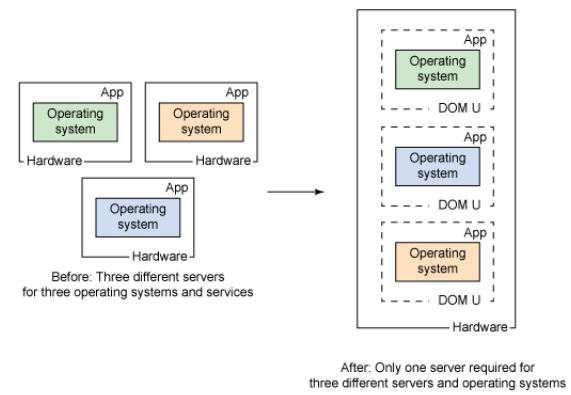
\includegraphics[width=1\textwidth]{figuras/virtualizacao.png}
\end{figure}


Os virtualizadores s�o componentes de software ou firmware capazes de virtualizar recursos f�sicos. Existem tr�s tipos de virtualiza��o diferentes, suas defini��es segundo \citeonline{tholeti2011hypervisors} s�o:

\begin{itemize}
	\item Tipo 1: a virtualiza��o de tipo 1 � caracterizada quando o virtualizador � executado diretamente sobre o hardware do sistema. Este m�todo � mais eficiente, tendo o melhor desempenho entre os m�todos de virtualiza��o;

	\item Tipo 2: a virtualiza��o de tipo 2 � caracterizada quando o virtualizador � executado sobre um sistema operacional hospedeiro que providencia servi�os de virtualiza��o, tais como suporte � entrada/sa�da de dados e gerenciamento de mem�ria;

	\item Virtualiza��o por uso de containers: este modo de virtualiza��o � caracterizado pela abstin�ncia do virtualizador. A virtualiza��o ocorre a n�vel de sistema operacional\abreviatura{SO}{Sistema Operacional} (SO), o qual permite a virtualiza��o de inst�ncias suas. Este modo de virtualiza��o resulta num uso mais eficiente de mem�ria, sendo esta sua vantagem diante dos outros m�todos de virtualiza��o. Todavia, como todas inst�ncias virtuais s�o imagens do SO ra�z, todas as inst�ncias ser�o da mesma vers�o que o SO ra�z.

\end{itemize}

A virtualiza��o � um processo utilizado nos ambientes na nuvem para dividir l�gicamente os recursos f�sicos de um servidor, normalmente sendo usados virtualizadores como componente respons�vel pela cria��o, remo��o e gerenciamento das \textit{virtual machines} \abreviatura{VM}{\textit{Virtual Machine}}(VMs), em portugu�s, m�quinas virtuais. O uso de virtualizadores facilita o provisionamento de diferentes sistemas operacionais sem que eles estejam instalados diretamente nos servidores f�sicos. Outra vantagem da virtualiza��o est� na facilita��o do processo de migra��o de VMs em tempo de execu��o para outros servidores fisicos, facilitando o processo de manuten��o.


\subsection{Orquestra��o}
Dadas a complexidade e heterogeneidade de ambientes de computa��o em nuvem, contendo in�meros componentes e vari�veis din�micas interligadas, a ger�ncia destes ambientes torna-se humanamente imposs�vel\\ \cite{forecasting}. Tendo isso em vista, ferramentas foram criadas com o objetivo de orquestrar a infraestrutura do ambiente, realizando a liga��o dos diferentes componentes como servidores de armazenamento, virtualiza��o e dispositivos de redes para prover a abstra��o de uma nuvem computacional.

\citeonline{gabriel} cita cinco componentes que comp�em as ferramentas dispon�veis para orquestra��o:
\begin{enumerate}
 \item Um gerente de identidades que realiza a ger�ncia das credenciais dos usu�rios (autentica��o e autoriza��o), possibilitando seguran�a na organiza��o da infraestrutura;
 \item Um gerente de aloca��o que aloca m�quinas virtuais quando s�o instanciadas, ligadas ou migradas;
 \item Um \emph{hypervisor} que � o componente que interage com diferentes virtualizadores, sendo respons�vel por enviar comandos para cada cluster;
 \item Um componente de armazenamento que realiza a distribui��o e o compartilhamento das unidades de armazenamento de m�quinas virtuais entre os servidores;
 \item Um elemento encarregado de gerenciar a configura��o da rede.
\end{enumerate}

A Figura \ref{fig:orquestracao}, retirada de \citeonline{gabriel}, apresenta um modelo gen�rico de ferramenta de orquestra��o.

 \begin{figure}[!htb]
 	\centering
 	\caption{Modelo de uma ferramenta de orquestra��o \cite{gabriel}.}\label{fig:orquestracao}
 	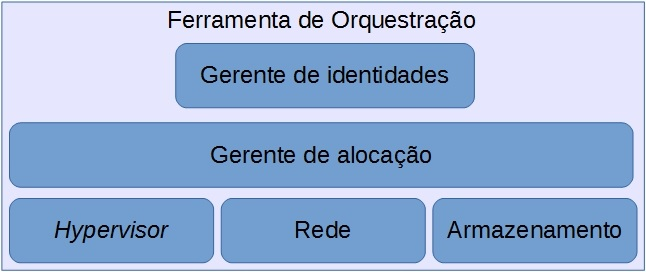
\includegraphics[scale=0.45]{figuras/ferramentasOrquestracao.jpg}
 \end{figure}

A ferramenta escolhida por \citeonline{gabriel}, que tamb�m ser� utilizada nesse trabalho, � o \textit{Cloudstack} \cite{cloudstack}. A escolha � motivada pelos fatos de que a ferramenta demonstra uma evolu��o constante num projeto que mant�m uma comunidade participativa, documenta��o completa e detalhada e o uso de tecnologias conhecidas para armazenamento de dados.


\subsection{Efici�ncia energ�tica e consolida��o}
Melhorar a efici�ncia energ�tica � uma das maiores dificuldades da computa��o em nuvem \cite{challenges}, sendo estimado que 53\% de todos os gastos de centro de processamento de dados s�o voltados a energia e refrigera��o \cite{micro-slice}. Aderindo a tend�ncias globais de busca de abordagens sustent�veis, surgiu a ideia de se buscar novas formas de diminuir o consumo de energia em ambientes de computa��o em nuvem, mantendo suporte a cargas din�micas e qualidade de servi�o.

Uma das estrat�gias encontradas para uma melhor efici�ncia energ�tica � a consolida��o. Assim como em \citeonline{gabriel}, no �mbito deste trabalho, consolida��o ser� tratada como a agrega��o de m�quinas virtuais em servidores f�sicos, de forma a concentrar um n�mero maior de m�quinas virtuais em um n�mero menor de servidores f�sicos. Essa forma de agrega��o permite a desativa��o de recursos ociosos, levando a um menor consumo energ�tico.

O benef�cio de t�cnicas de consolida��o vem na possibilidade de aumentar a efici�ncia de um ambiente de CN atrav�s do desligamento de recursos ociosos. Em um cen�rio �timo, todos os servidores que est�o ligados, tendem a carga m�xima, fazendo com que a efici�ncia deste ambiente tamb�m esteja tendendo ao m�ximo poss�vel. Para que seja poss�vel a consolida��o, deve ser poss�vel migrar VMs em tempo de execu��o, fato que s� ocorre entre servidores com hardware compat�vel e mesmo virtualizador. Este e outros fatores, como a necessidade de atender a cargas estoc�sticas, faz com que a consolida��o de ambientes em nuvem n�o seja um problema trivial de se resolver.\par

Para que a consolida��o seja poss�vel, deve haver alguma forma de comunica��o entre servidores, para que estes acordem em realizar um rebalanceamento de carga. Al�m disso, a comunica��o e migra��o deve ocorrer entre m�quinas que se encaixam no cen�rio em que h� a necessidade de uma migra��o em tempo de execu��o. Neste tipo de ambiente, al�m de estarem presentes conceitos de negocia��o e atos de fala, h� informa��o fragmentada inserida nos elementos do ambiente. Tais pontos s�o discutidos e est�o presentes no conjunto de caracter�sticas de problemas onde o uso de sistemas multiagente � recomendado, apontadas por Wooldridge em seu livro \cite{wooldridge2009introduction}.


\subsection{Sistemas Multiagentes}
Sistemas multiagentes � considerada uma �rea de estudo dentro da Intelig�ncia Artificial Distribu�da (IAD)\abreviatura{IAD}{Intelig�ncia Artificial Distribu�da}. SMA possuem a capacidade de lidar com problemas em ambientes distribu�dos e abertos, tal como os ambientes em larga escala encontrados que usam a internet como meio \cite{wooldridge2009introduction}.\par

A abordagem de SMA � descrita na forma de m�ltiplos elementos computacionais (agentes) que trocam conhecimento entre si na forma de coopera��o, coordena��o, negocia��o e similares, possibilitando a fragmenta��o de problemas complexos em sub-problemas menores e objetivos. Estes, por sua vez, podem ser abordados de diferentes formas, por diferentes agentes especialistas \cite{a-ricardo-intro}.\par

O emprego de SMA tem apresentado sucesso em �reas que trabalham com ambientes din�micos e descentralizados, onde a tomada de decis�o n�o depende apenas de um �nico ponto de vista \cite{kelash2007takes}.

\subsection{Agentes}
% LUCAS

 Agentes s�o entidades capazes de se comunicar entre si, possuem mobilidade e comportam-se de forma independente e inteligente dentro do ambiente. Um agente � um sistema computacional capaz de atuar autonomamente de maneira a alcan�ar seus objetivos \cite{wooldridge2009introduction}. Seu conceito pode ser  abstraido para uma entidade auto-contida, capaz de interagir (atrav�s de fun��es atuadoras e sensoras) com o 
ambiente em que se encontra, consigo mesma e com outros agentes \cite{ia-ferramentas}. Ter v�rios agentes em um sistema implica que cada agente deve raciocinar e agir levando em considera��o os outros agentes no sistema, sendo que dentro de um sistema, diferentes agentes podem ou n�o ter um prop�sito em comum \cite{handbook-knowledge}. Este segundo caso � particularmente interessante, j� que as diferentes entidades podem ter o mesmo objetivo, mas diferentes crit�rios, possivelmente conflitantes, a priorizar na satisfa��o de suas metas. Independente de seu tipo e ambiente, agentes funcionam em um ciclo cont�nuo de perceber o mundo, decidir sua pr�xima a��o e execut�-la. A Figura \ref{fig:agente} representa o ciclo cont�nuo de execu��o de um agente. 

\begin{figure}[!htb]
	\centering
	\caption{Representa��o de um agente em um ambiente, obtido de \cite{RussellLivro}.}\label{fig:agente}
	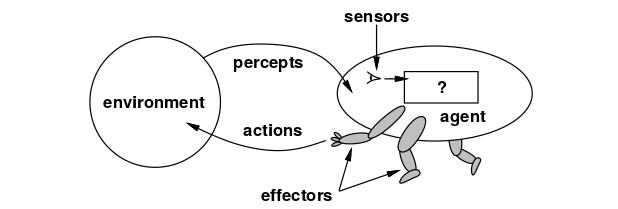
\includegraphics[width=1\textwidth]{figuras/imgAgent.png}
\end{figure}

Agentes possuem m�dulos que servem como sensores e atuadores, representando sua interface com o mundo. Eles est�o diretamente relacionados com as capacidades dos agentes de perceber e agir. Atrav�s dos sensores, um agente consegue perceber o ambiente que ele est� inserido. Esta entrada, na forma percep��es, � avaliada pelo agente, resultando em uma decis�o de a��o. Por fim, atrav�s dos atuadores, o agente � capaz de agir em seu ambiente, modificando o estado do ambiente.

\subsubsection{Caracter�sticas de Agentes}

Um agente � respons�vel por representar um ponto de vista e agir de forma coerente para alcan�ar um objetivo. Assim como uma sociedade de agentes exprime v�rios pontos de vista e objetivos. No evento em que dois ou mais pontos de vista entram em conflito, os agentes devem ter a capacidade de negociar, para que possam encontrar a melhor a��o para o problema em conjunto \cite{wooldridge2009introduction}.\par 

Segundo Silveira em \cite{a-ricardo-intro}, mesmo tendo natureza diversa, os agentes possuem caracter�sticas recorrentes, relacionadas com suas abordagens para resolver problemas e capacidade de comunica��o. Encontrado em maior ou menor grau em uma implementa��o de um agente, estes atributos s�o:

\begin{itemize}  
	\item Reatividade: a habilidade de perceber o ambiente de modo seletivo e manifestar um
	comportamento como resposta a um est�mulo externo;
	\item Autonomia: comportamento dirigido a objetivos, pr�-ativo e auto-iniciado;
	\item Comportamento cooperativo: trabalhar com outros agentes para atingir um objetivo
	comum;
	\item Habilidade de comunica��o ao n�vel de conhecimento: capacidade de comunicar-se com
	pessoas ou outros agentes em uma linguagem de mais alto n�vel que um simples protocolo
	de comunica��o programa a programa;
	\item Capacidade de infer�ncia: capacidade de agir a partir de especifica��es abstratas de
	tarefas, usando conhecimentos pr�vios;
	\item Continuidade temporal: persist�ncia de identidade por longos per�odos de tempo;
	\item Personalidade: capacidade de demonstrar atributos de um personagem;
	\item Adaptabilidade: habilidade de aprender com a experi�ncia;
	\item Mobilidade: habilidade de migrar de uma plataforma para outra.
\end{itemize}

As diferen�as entre agentes � o fator respons�vel pela heterogeniedade do SMA. O fato de que diferentes entidades dividem o mesmo ambiente, faz com que um problema possa ser percebido de diferentes formas e lidado de maneiras diferentes e condizentes com um plano de a��o conjunto. Em adi��o � suas caracter�sticas, os agentes possuem estrat�gias diferentes para a tomada de decis�o, fator que gera diferentes classifica��es para estes, descritas nas pr�ximas sub-se��es.

\subsubsection{Agentes Reativos}

Segundo \citeonline{wooldridge2009introduction}, agentes puramente reativos s�o entidades computacionais que decidem suas a��es baseados exclusivamente no estado presente do ambiente. Eles recebem seu nome em raz�o do comportamento an�logo a uma resposta imediata, sem consulta a um hist�rico passado de conhecimento. Essa abordagem � focada no que os agentes podem realizar, juntos ou separadamente, sem existir necessariamente mem�ria ou comunica��o direta entre eles. Nesse caso, agentes tomam conhecimento de a��es e comportamentos de outros 
agentes apenas atrav�s de modifica��es no ambiente \cite{ia-ferramentas}. Embora sejam �teis em raz�o de que s�o programados de forma a ter comportamentos hierarquicamente organizados, esse tipo de agente pode se tornar muito complexo para entender quando o n�mero de comportamentos associado a eles cresce.

\subsection{Agentes Deliberativos}

Agentes deliberativos s�o aqueles que tem alguma forma de reten��o de conhecimento na forma de experi�ncias passadas, criando um modelo expl�cito de mundo. Estes agentes tamb�m possuem uma expl�cita representa��o de outros agentes, mem�ria (que 
permite que os agentes plenejem suas a��es tendo eventos passados como base) e capacidade de se comunicarem diretamente uns com os outros. Esse modelo de agente � mais focado nas atitudes que os caracterizam, sendo que com o tempo, realizando diferentes intera��es com os sistemas, estes devem desenvolver cren�as (no sentido de reconhecer padr�es), inten��es, entre outras caracter�sticas de uma entidade racional com a finalidade de auxiliar a escolha de seus planos de a��o futuros, suplementando sua percep��o atual do ambiente \cite{handbook-knowledge}.\par

No contexto de um agente cognitivo, um conjunto de cren�as � chamado de banco de conhecimento. Esse � continuamente atualizado com as percep��es do agente, assim como � usado para verificar condi��es necess�rias para a escolha de um pr�ximo plano de a��o do agente. Na Figura \ref{fig:agente-BDI} pode-se observar a arquitetura de um agente deliberativo que age no formato de \textit{Beliefs, Desire and Intentions} \abreviatura{BDI}{Beliefs Desire Intentions}(BDI), em portugu�s cren�as, desejos e inten��es.

\begin{figure}[!htb]
	\centering
	\caption{Modelo gen�rico de um agente deliberativo BDI, obtido de \cite{bdi4jade}.}\label{fig:agente-BDI}
	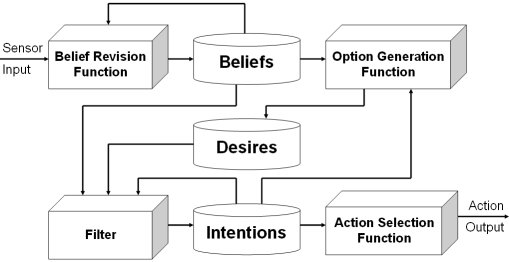
\includegraphics[width=1\textwidth]{figuras/bdiArch.jpg}
\end{figure}

Os agentes BDI s�o aqueles que mant�m uma s�rie de objetivos, armazenados na forma de desejos, mant�m planos na forma de inten��es e possuem cren�as, que s�o informa��es que guardam de forma simb�lica sobre o ambiente. Utilizando l�gica de predicados de primeira ordem, um agente BDI pode escolher qual plano melhor se encaixa na sua vis�o de mundo atual.

\subsubsection{Agentes H�bridos}

De acordo com \cite{wooldridge2009introduction}, agentes h�bridos s�o capazes de apresentar comportamento reativo e proativo atrav�s da modelagem de camadas de comportamentos. A partir dos dados providos pela leitura do ambiente, o agente pondera seus comportamentos da camada de planos reativos e da sua camada de comportamentos proativos. A sa�da dessa fun��o de pondera��o � interpretada de forma an�loga a uma sugest�o de plano. Agentes deste tipo funcionam gra�as a presen�a expl�cita ou n�o de uma camada de controle de comportamentos.

\subsection{Modelagem de Sistemas de Agentes}
Sistemas baseados em agentes podem ser modelados de forma similar a sistemas orientados a objeto, sendo que seus agentes tomam forma de objeto e passam a ser constitu�dos por atributos e m�todos podendo se comunicar invocando m�todos de outros agentes ou trocando mensagens, e podendo utilizar conceitos cl�ssicos de orienta��o a objeto, como heran�a, encapsulamento e agrega��o de dados \cite{intelligent}. Em consequ�ncia disso, m�todos relacionados ao desenvolvimento de aplicativos orientados a objeto formam a base de boa parte dos m�todos de desenvolvimento de sistemas baseados em agentes. De forma similar a t�cnica para modelagem orientada a objeto proposta por \citeonline{OMT} que consiste de modelo b�sico, modelo est�tico e modelo din�mico, \citeonline{agent-oriented} divide a an�lise orientada a agentes em tr�s modelos, o modelo de agente, o modelo organizacional e o modelo cooperativo, descritos a seguir:

\begin{itemize}
  \item O modelo de agente cont�m descri��es e estruturas internas dos agentes, descritas em termos de no��es mentais como metas planos e cren�as ou quaisquer estruturas que sejam apropriadas a arquitetura espec�fica dos agentes sendo desenvolvidos. Esse modelo se assemelha ao modelo b�sico de m�todos de orienta��o a objeto;
  \item O modelo organizacional especifica os relacionamentos entre agentes e seus tipos. Estes s�o em parte rela��es de heran�a, e tamb�m relacionamentos entre agentes baseados em seus respectivos pap�is em organiza��es. Essas organiza��es podem ser meios para estruturar sistemas complexos em subsistemas (assim como � feito em certas t�cnicas de orienta��o a objeto) ou podem ser usadas para modelar organiza��es reais. Esse modelo � semelhante ao modelo est�tico, mas como pap�is podem mudar com o passar do tempo, ele n�o � um modelo genuinamente est�tico;
  \item O modelo cooperativo descreve a intera��o, ou mais especificamente, a coopera��o entre os agentes. Este modelo cont�m apenas os \hyphenation{relacio-namentos} relacionamentos entre objetos. O processo que ocorre dentro dos objetos � representado pelo modelo de agente.
\end{itemize}


\subsection{Comunica��o de Agentes}
A coopera��o e a comunica��o entre agentes torna-se interessante quando existe a inten��o de resolver um problema de forma distribu�da, como � o caso da orquestra��o de um ambiente de computa��o em nuvem. Existem v�rios m�todos de comunica��o entre agentes fundamentalmente diferentes, sendo que \citeonline{intelligent} classificam como o mais simples dos m�todos a invoca��o do procedimento de um agente por outro agente.

Utilizando a invoca��o de procedimentos, o agente invocador (agente 1) usa par�metros de invoca��o expl�citos para informar o outro agente (agente 2) de suas inten��es. Os valores de retorno do agente 2 representam a resposta da comunica��o. Por�m, apenas comunica��es muito simples podem ser efetuadas invocando procedimentos remotos, sendo que para casos com um m�nimo de complexidade os m�todos de comunica��o entre agentes podem ser diferenciados em sistemas \emph{blackboard} (quadro negro) e sistemas baseados em di�logo (troca de mensagens) \cite{intelligent}.

O conceito de quadro negro surgiu a partir da inten��o de lidar com aplica��es complexas e fracamente definidas, dando mais flexibilidade a pesquisadores e desenvolvedores, liberando-os de especifica��es formais excecivas \cite{blackboard}. Um quadro negro proporciona a todos os agentes dentro de um sistema uma �rea comum de trabalho, a qual eles podem utilizar para trocar informa��es \cite{intelligent}. Um agente inicia a comunica��o escrevendo um item de informa��o qualquer no quadro negro. Este item fica ent�o dispon�vel para todos os outros agentes do sistema, sendo que qualquer agente pode acessar o quadro negro a qualquer momento para verificar se novas informa��es surgiram desde sua �ltima verifica��o \cite{intelligent}. Neste modelo os agentes n�o precisam saber dos conhecimentos e nem da exist�ncia dos outros agentes dentro do sistema, mas devem ser capazes de compreender as informa��es contidas no quadro negro \cite{blackboard}.

A alternativa ao quadro negro vem na forma de troca de mensagens. A comunica��o via troca de mensagens proporciona uma base flex�vel para a implementa��o de estrat�gias complexas de coordena��o de agentes, sendo que as mensagens trocadas entre os agentes podem ser usadas para estabelecer comunica��es e mecanismos de coopera��o usando protocolos pr�-definidos \cite{intelligent}. O fato de que diferentes agentes podem ser invocados para realizarem fun��es diferentes dentro do ambiente, mas em algum ponto de suas respectivas fun��es, necessitar de alguma informa��o da qual outro agente pode ter conhecimento \cite{handbook-intelligence} � algo que torna essa abordagem interessante em um ambiente de computa��o em nuvem.

